\documentclass[14,fleqn]{article}
\usepackage{amsmath}
\usepackage{amssymb}
\usepackage[top=.5 in,left=.5 in,right=.5 in,bottom=.5 in]{geometry}
\usepackage{enumerate}
\usepackage{ mathrsfs }
\usepackage{graphicx}
\usepackage{pgf,tikz}
\usepackage{mathrsfs}
\usepackage{gensymb}
\usepackage{venndiagram}
\usetikzlibrary{arrows}

\pagenumbering{gobble}

\setlength{\parindent}{0 pt}
\setlength{\parskip}{1 ex}

\newcommand{\lcm}{\textnormal{lcm}}
\newcommand{\norm}{\triangleabove right}
\newcommand{\bfm}[1]{$\boldsymbol{#1}$}
\newcommand{\Z}{\ensuremath{\mathbb{Z}}}
\newcommand{\R}{\ensuremath{\mathbb{R}}}
\newcommand{\C}{\ensuremath{\mathbb{C}}}
\renewcommand{\wedge}[1]{\ensuremath{\langle #1 \rangle}}
\newcommand{\infsum}[1]{\ensuremath{\sum_{n=#1}^\infty}}
\newcommand{\defn}[1]{\textbf{\underline{#1}}}

%\begin{venndiagram3sets}[labelA=$S$,labelB=$T$,labelC=$U$]
%	\fillA
%	\fillOnlyC
%\end{venndiagram3sets}\\

%\begin{venndiagram2sets}[labelA=$S$,labelB=$T$]
%	\fillNotA
%	\fillNotB
%	\setpostvennhook{
%		\draw[] (labelAB) ++(0,-2.1) node {\raisebox{0pt}[0pt][0pt]{$(S\cap T)'$}};
%	}
%\end{venndiagram2sets}\\

\begin{document}
\section{Section 6.3: Assignment of Probabilities}
Suppose we have an experiment with sample space $S$ of size $N$ consisting of equally likely outcomes. Then for some event $E=\{s_1,\dots,s_k\}$ we must have
\[
	P(E)=P(s_1)+\cdots +P(s_k)=\underbrace{\frac{1}{N}+\cdots + \frac{1}{N}}_{k \mathrm{ times}}=\frac{k}{N}=\frac{n(E)}{n(S)}
\]
So in experiments with equally likely outcomes, we use our counting principles to count the size of the event and sample space.

Example: Suppose an urn has 5 red balls, 4 green balls, and 3 white balls in it. Three balls are picked from the urn randomly and without replacement.
\begin{enumerate}
	\item What is the probability that all 3 balls are green?
	\item What is the probability that at least 1 ball is white?
	\item What is the probability the 3 balls are different colors?
	\item What is the probability that each ball is the same color?
\end{enumerate}

Solutions:\\
\begin{enumerate}
	\item First we have to calculate the size of the sample space. Since there are 12 balls and we are choosing 3 we know that there are $\binom{12}{3}=220$ possible ways to choose the balls. If we want all 3 of them to be green there are exactly $\binom{4}{3}=4$ ways to choose 3 green balls. Thus the probability of choosing all green balls is $4/220=1/55.$
	\item The sample space is the same for each question so we know there are 220 possible outcomes. So now we need to find how many ways to choose balls so at least one of them is white. We could do this directly or we could use the complement rule. The complement of at least 1 being white is that none are white. Since there are 9 balls that aren't white there are $\binom{9}{3}=84$ ways to choose balls so that none of them are white. Thus there are $220-84=136$ ways to choose balls so that at least 1 is white. Thus the probability that at least 1 ball is white is $136/220=34/55.$
	\item If the 3 balls are different colors then we simply need to choose 1 of each. Since there are 5 red, 4 green, and 3 white. There are $5\cdot 4\cdot 3=60$ ways to choose 1 ball of each color. Thus the probability is $60/220=3/11.$
	\item If all the balls are the same color then they must be all red, all green or all white. We know that there are $\binom{4}{3}$ ways to get them all green. There are $\binom{5}{3}=10$ ways to choose all red, and there are $\binom{3}{3}=1$ ways to choose all white. Thus there are $1+4+10=15$ ways to choose all of the same color. So the probability is $15/220=3/44.$
\end{enumerate}

Let's take a closer look at question 2. We used the complement rule to count the size of the event. But let's look at what's really going on. Suppose $E$ is some event then we get
\[
	P(E')=\frac{n(E')}{n(S)}=\frac{n(S)-n(E)}{n(S)}=1-\frac{n(E)}{n(S)}=1-P(E')
\]
This is called the \defn{complement rule} for probability. Notice the similarity to the set rule. Note this is always true by inclusion exclusion for probability.\\

A company makes smart phones and sends them out in boxes of 10. For quality control, 4 phones are selected from each box to see if they are defective in any way. The box is not sent if one of the 4 phones is defective. What is the probability the box is not sent if there is 1 defective phone in the box? What if there are 2 defective phones?\\

In either case there are $\binom{10}{4}=210$ ways to choose the phones. Also, in either case we will use the complement rule. If there is 1 defective phone then there are $\binom{9}{4}=126$ to choose so that none are defective. So the probability of not choosing a defective phone is $126/210.$ Thus the probability of not sending the box is $1-126/210=84/210.$ If there are 2 defective phones then there are $\binom{8}{4}=56$ ways to choose them. Thus there is probability $1-56/210=154/210$ that the box will not be sent.\\

The previous example shows why quality control works. We don't have to test every unit to be fairly confident that all units work correctly.\\

Example: Birthday Paradox\\
Suppose there are 5 people in a room. What is the probability that at least 2 share a birthday. What if there are 10 people. How many people do you need to have a greater than $1/2$ chance that two share a birthday.\\

The complement of the event is that all 5 have different birthdays. There are $365^5$ possibilites for birthdays. If each has a different one then there are $365\cdot 364\cdot 363\cdot 362\cdot 361$ ways to choose them thus the probability is
\[
	1-\frac{365\cdot 364\cdot 363\cdot 362\cdot 361}{365^5}=0.027
\]

We do the same calculations for 10 people and get a $0.117$ probability. It turns out that you only need 23 people to have a greater than $1/2$ probability.

Example: Consider the following map of a city grid.\\
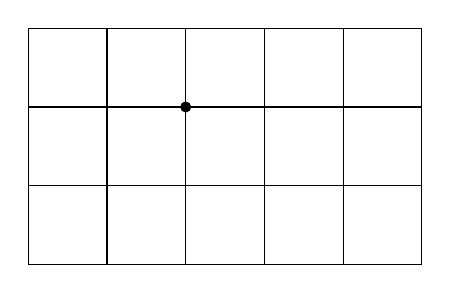
\begin{tikzpicture}
	\draw[step=1.0, black, thin] (0,0) grid (5,3);
	\fill (2,2) circle[radius=2 pt];
\end{tikzpicture}\\
What is the probability that a random shortest path will go through the given point. What is the probability that a random shortest path will go up as its last step. What is the probability that a random shortest path will never go up twice in a row.\\

For each of these questions we need to know how many shortest paths there are. We can recall this equivalent to choosing 3 of the 8 moves where we go up. Thus there are $\binom{8}{3}=56$ possible shortest paths.\\

How many will go throught the given point. This means we first make a shortest path to the given point then make a shortest path after. Thus there are $\binom{4}{2}\binom{4}{1}=24$ paths through the given point. So the probability is $24/56=3/7.$\\

If the path goes up as the last step the we basically have to find a shortest path to the space below. This is the same as drawing a differnt dot to go through where there are no choices after. There are $\binom{7}{2}=21$ possible paths so the probability is $21/56=3/8.$\\

To count the number of paths that never go up twice in a row we use the trick where we line up the rights and put ups in between them, one per spot. There are 3 ups and 6 spots so there are $\binom{6}{3}=20$ possible paths. So the probability is $20/56=5/14.$

Things to watch out for:
\begin{enumerate}
	\item In the lottery (3 numbers 0-9 in order) what is the probability of 000
	\item what is the probability of a ``random number like 384 (same)
	\item if you flip a coin 4 times in a row what is the probability of 4 heads
	\item what is the probability of getting THTT (same)
	\item If you flip a fair coin 100 times in a row and get all heads, what is the probability that flip 101 is a head (1/2)
\end{enumerate}


\end{document}
